\clearpage
\section{Voice flow}
\label{sec:voice_flow}
È resa disponibile all'utente una skill utilizzabile con l'assistente Amazon Alexa che permette l'avvio dei workflow presenti nell'applicazione tramite comandi vocali.
L'immagine sottostante rappresenta lo schema di un Voice flow generico avviato tramite la skill.
\begin{figure}[H]
	\centering
	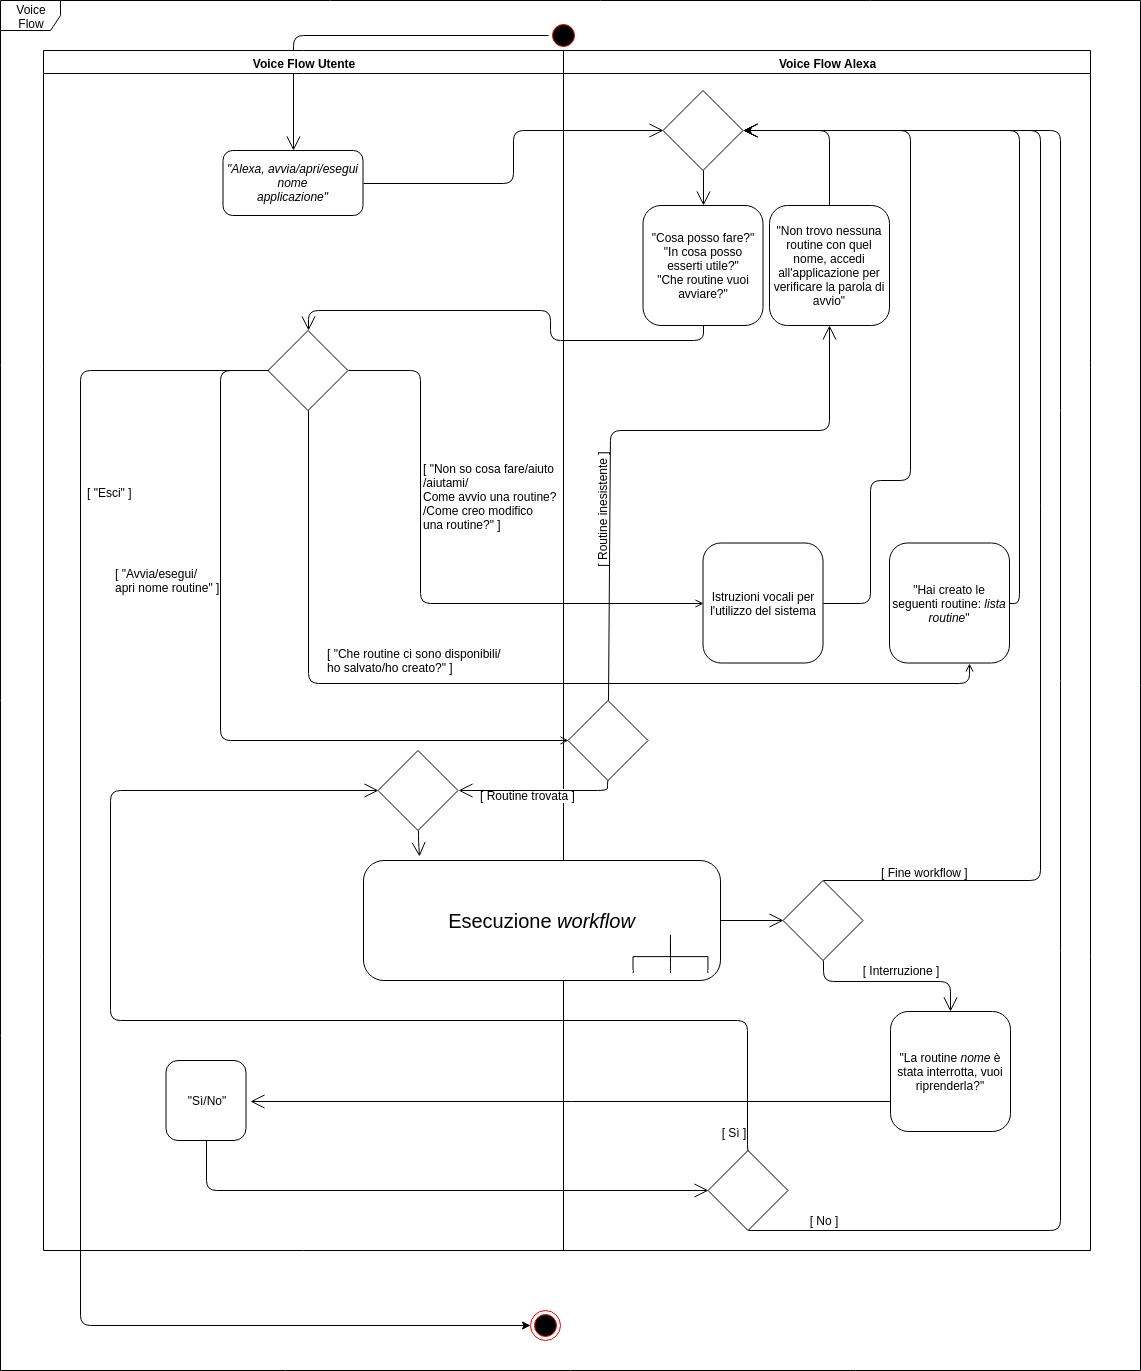
\includegraphics[width=15cm,keepaspectratio]{../includes/pics/voice_flow_alexa-utente_UML.png}
	\caption{\label{fig:mission}Schema Voice flow generico}
\end{figure}
\begin{figure}[H]
	\centering
	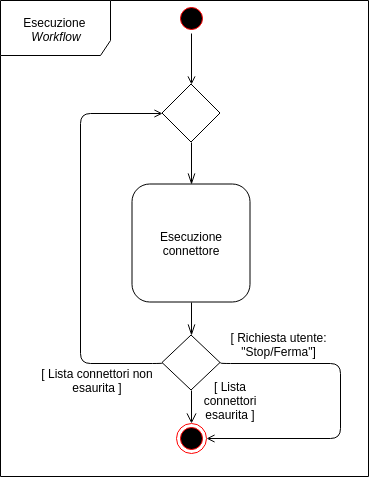
\includegraphics[height=12cm]{../includes/pics/esecuzione_connettore.png}
	\caption{\label{fig:mission}Schema Voice flow generico}
\end{figure}
\subsection{Interazione vocale utente - Assistente vocale}
\label{sec:iterazione_vocale_utente}
Durante l'esecuzione del workflow alcuni connettori potrebbero necessitare di un'ulteriore interazione vocale tra l'utente e l'assistente vocale. Di seguito viene esplicato in che modo è strutturato il dialogo tra l'utente e Amazon Alexa.
\subsection{Interazioni UC18 - Connettore: imposta sveglia}
\label{sec:connettore_sveglia}
\begin{itemize}
        \item Alexa: "Vuoi/Desideri impostare una sveglia?".
        \item Utente: "Sì/No/{\it orario}".
        \begin{itemize}
         \item{Risposta {\it "Sì"} }, Alexa:"Che orario vuoi impostare per la sveglia?".
         \begin{itemize}
              \item{Risposta {\it orario} corretto}, Alexa:"La sveglia è stata impostata alle ore {\it orario}".
              \item{Risposta {\it orario} errato}, Alexa:  {\it UC18.2 - Ricezione notifica orario errato}
         \end{itemize}
         \item{Risposta {\it "No"} }, il sistema passa al connettore successivo o termina il workflow se non sono presenti altri connettori.
         \item{Risposta {\it orario} corretto}, Alexa:"La sveglia è stata impostata alle ore {\it orario}".
         \item{Risposta {\it orario} errato}, Alexa:  {\it UC18.2 - Ricezione notifica orario errato}
         \end{itemize}
    \end{itemize}

\subsection{Interazioni UC19 - Connettore: riproduzione musica}
\label{sec:connettore_musica}
 \begin{itemize}
        \item Alexa: "Cosa/chi vuoi ascoltare?".
        \item Utente: "{\it nome artista}/{\it nome traccia}".
        \begin{itemize}
         \item{Risposta {\it nome artista} corretto}, il sistema fa riprodurre ad Alexa le tracce dell'artista.
        \item{Risposta {\it nome artista} errato}, Alexa:  {\it UC19.1 - Ricezione notifica titolo o artista non riconosciuto}.
        \item{Risposta {\it nome traccia} corretto}, il sistema fa riprodurre ad Alexa la traccia.
        \item{Risposta {\it nome traccia} errato}, Alexa:  {\it UC19.1 - Ricezione notifica titolo o artista non riconosciuto}.
         \end{itemize}
    \end{itemize}


\subsection{Interazioni UC21 - Connettore: lettura calendario}
\label{sec:connettore_lettura_calendario}
\begin{itemize}
        \item Alexa: "Domani hai fissato i seguenti eventi: {\it lista eventi}, vuoi sapere gli eventi del resto della settimana?".
        \item Utente: "Sì/No".
        \begin{itemize}
         \item{Risposta "Sì"}, Alexa: "Hai fissato i seguenti eventi: {\it lista eventi successivi}".
         \item{Risposta "No"}, il sistema passa al connettore successivo o termina il workflow se non sono presenti altri connettori.
         \end{itemize}
    \end{itemize}


\subsection{Interazioni UC22 - Connettore: aggiunta evento calendario}
\label{sec:connettore_evento_calendario}
 \begin{itemize}
        \item Alexa: "Vuoi aggiungere un evento?".
        \item Utente: "Sì/No".
        \begin{itemize}
         \item{Risposta "Sì"}, Alexa: "In che data?".
         \item Utente: "{\it data}".
         \begin{itemize}
             \item{Risposta {\it data in formato corretto}}, Alexa: "Che nome vuoi dare all'evento?".
             \item Utente: {\it nome evento}.
             \item Alexa: "Ho creato l'evento {\it nome evento} in data {\it data}."
            \item{Risposta "{\it data in formato non corretto}}, Alexa: {\it UC22.1 - Ricezione notifica data errata}.
         \end{itemize}
         \item{Risposta "No"}, il sistema passa al connettore successivo o termina il workflow se non sono presenti altri connettori.
         \end{itemize}
    \end{itemize}

\subsection{Interazioni UC23 - Connettore: scrittura nota}
\label{sec:connettore_nota}
\begin{itemize}
        \item Alexa: "Vuoi aggiungere una nota?".
        \item Utente: "Sì/No".
        \begin{itemize}
         \item{Risposta "Sì"}, Alexa: "Dimmi pure/Che nota aggiungo?".
         \item Utente: "{\it Corpo nota}".
         \item{Risposta "No"}, il sistema passa al connettore successivo o termina il workflow se non sono presenti altri connettori.
         \end{itemize}
    \end{itemize}


\subsection{Interazioni UC24 - Connettore: pubblicazione e lettura Tweet}
\label{sec:connettore_twitter}
 \begin{itemize}
        \item Alexa: "Cosa vuoi fare? Puoi: pubblicare un tweet, leggere i tweet di {\it Account impostato da connettore}, leggere i tweet della tua bacheca".
        \item Utente: "Voglio pubblicare un tweet/Voglio leggere i tweet di {\it Account impostato da connettore}/Voglio leggere i tweet della mia bacheca".
        \begin{itemize}
         \item{Risposta "Voglio pubblicare un tweet"}, Alexa: "{\it UC24.1 - Pubblicazione tweet}".
         \item{Risposta "Voglio leggere i tweet di {\it Account impostato da connettore}"}, Alexa: "{\it UC24.2 - Lettura ultimi tweet da singolo account}".
         \item{Risposta "Voglio leggere i tweet della mia bacheca"}, Alexa: "{\it UC24.3 - Lettura tweet bacheca personale}".
         \end{itemize}
    \end{itemize}


\subsection{Interazioni UC24.1 - Pubblicazione tweet}
\label{sec:connettore_twitter_scrittura}
\begin{itemize}
        \item Alexa: "Dimmi pure cosa vuoi pubblicare./Cosa vuoi rispondere?".
        \item Utente: "{\it corpo tweet}".
        \begin{itemize}
        \item Alexa: "Ho pubblicato il tuo tweet".
           \end{itemize}
        \item Utente: "{\it corpo tweet con più di 280 caratteri}".
           \begin{itemize}
        \item Alexa: "{\it UC24.1.1 - Ricezione notifica fine caratteri disponibili}".
           \end{itemize}
        
    \end{itemize}


\subsection{Interazioni UC24.2 - Lettura ultimi tweet da singolo account}
\label{sec:connettore_twitter_profilo}
 \begin{itemize}
        \item Alexa: "Gli ultimi tweet di {\it Account impostato da connettore} sono {\it lettura corpo tweet}".
        \item Utente che interrompe dopo l'ascolto di un tweet: "Voglio rispondere".
        \item Alexa: "{\it UC24.1 - Pubblicazione tweet}".
    \end{itemize}


\subsection{Interazioni UC24.3 - Connettore: lettura tweet bacheca personale}
\label{sec:connettore_twitter_bacheca}
 \begin{itemize}
        \item Alexa: "Nella tua bacheca ho trovato i seguenti tweet: {\it lettura corpo tweet}".
        \item Utente che interrompe dopo l'ascolto di un tweet: "Voglio rispondere".
        \item Alexa: "{\it UC24.1 - Pubblicazione tweet}".
    \end{itemize}


\subsection{Interazioni  UC25 - Connettore: operazioni con Trello}
\label{sec:connettore_trello} 
 \begin{itemize}
        \item Alexa: "Cosa desideri fare nella bacheca {\it bacheca impostata}? Puoi: leggere le tue schede, aggiungere una nuova scheda, spostare una scheda tra liste".
        \item Utente: "Voglio leggere le mie schede/Voglio aggiungere una scheda/Voglio spostare una scheda.".
        \begin{itemize}
         \item{Risposta "Voglio leggere le mie schede"}, Alexa: "{\it UC25.1 - Lettura lista da bacheca Trello}".
         \item{Risposta "Voglio aggiungere una scheda"}, Alexa: "{\it  UC25.2 - Creazione scheda in bacheca Trello}".
         \item{Risposta "Voglio spostare una scheda"}, Alexa: "{\it UC25.3 - Spostamento scheda tra liste Trello}".
         \end{itemize}
    \end{itemize}


\subsection{Interazioni UC25.1 - Lettura lista da bacheca Trello}
\label{sec:connettore_trello_leggi_bacheca}
 \begin{itemize}
        \item Alexa: "Che lista devo leggere?".
        \item Utente: "{\it nome lista esistente}".
        \begin{itemize}
        \item Alexa: "{\it lettura lista}".
           \end{itemize}
        \item Utene: "{\it nome lista inesistente}".
           \begin{itemize}
        \item Alexa: "{\it UC25.6 - Ricezione notifica lista inesistente}".
           \end{itemize}
    \end{itemize}


\subsection{Interazioni UC25.2 - Creazione scheda in bacheca Trello}
\label{sec:connettore_trello_crea_bacheca}
 \begin{itemize}
        \item Alexa: "In che lista vuoi che aggiunga la scheda?".
        \item Utente: "{\it nome lista esistente}".
        \begin{itemize}
        \item Alexa: "Dimmi pure".
        \item Utente: "{\it corpo scheda}".
           \end{itemize}
        \item Utente: "{\it nome lista inesistente}".
           \begin{itemize}
        \item Alexa: "{\it UC25.6 - Ricezione notifica lista inesistente}".
           \end{itemize}
    \end{itemize}


\subsection{Interazioni  UC25.3 - Spostamento scheda tra liste Trello}
\label{sec:connettore_trello_sposta_scheda}
 \begin{itemize}
        \item Alexa: "Da che lista vuoi spostare la scheda?".
        \item Utente: "{\it nome lista esistente}".
        \begin{itemize}
        \item Alexa: "Che scheda vuoi spostare".
       
        \item Utente: "{\it nome scheda esistente}".
        \begin{itemize}
        \item Alexa: "In che lista vuoi spostare la scheda?"
          \item Utente: "{\it nome lista esistente}".
          \begin{itemize}
              \item Alexa: "Scheda spostata con successo".
          \end{itemize}
           \item Utente: "{\it nome lista inesistente}".
           \begin{itemize}
        \item Alexa: "{\it UC25.6 - Ricezione notifica lista inesistente}".
        \end{itemize}
      \end{itemize}
      
     \item Utente: "{\it nome scheda inesistente}".
     \begin{itemize}
           \item Alexa: "{\it UC25.3.1 - Ricezione notifica scheda inesistente}".
           \end{itemize}
            \end{itemize}
        \item Utente: "{\it nome lista inesistente}".
           \begin{itemize}
        \item Alexa: "{\it UC25.6 - Ricezione notifica lista inesistente}".
           \end{itemize}
    \end{itemize}
